\documentclass[tikz,border=6pt]{standalone}
\usepackage{lmodern}\usepackage[T1]{fontenc}
\definecolor{c3}{HTML}{D62828}
\definecolor{c4}{HTML}{F77F00}
\definecolor{c5}{HTML}{E9C000}
\definecolor{c6}{HTML}{2A9D3F}
\definecolor{c7}{HTML}{1F5FBF}
\definecolor{stB}{HTML}{4A4E53}
\begin{document}
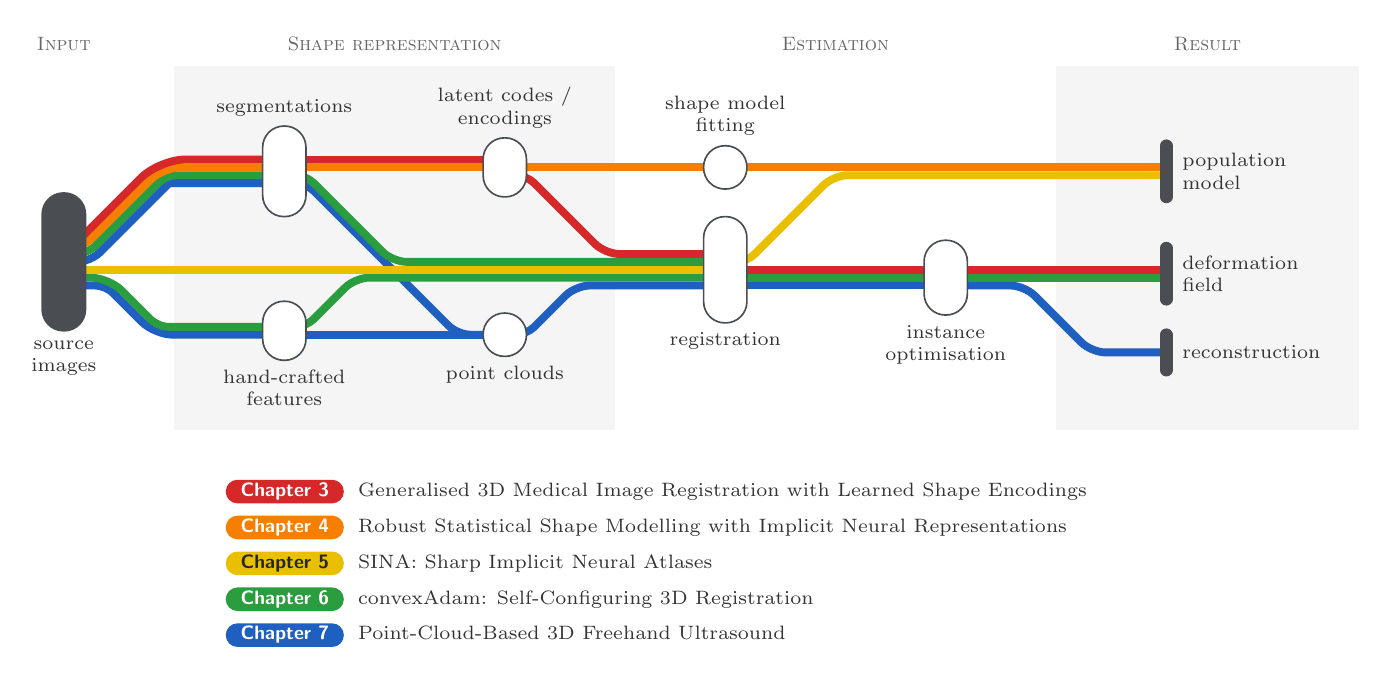
\begin{tikzpicture}[
  stn/.style={draw=stB, fill=white, line width=0.6pt, rounded corners=0.27cm},
  rt/.style={line width=0.10cm, line cap=butt, line join=round},
  lbl/.style={font=\scriptsize, align=center, text=black!80, inner sep=0pt}]
% ---- phase bands ----
\node[font=\scriptsize\scshape, text=black!60, anchor=south] at (0.000,2.415) {Input};
\fill[black!4] (1.400,-2.280) rectangle (7.000,2.335);
\node[font=\scriptsize\scshape, text=black!60, anchor=south] at (4.200,2.415) {Shape representation};
\node[font=\scriptsize\scshape, text=black!60, anchor=south] at (9.800,2.415) {Estimation};
\fill[black!4] (12.600,-2.280) rectangle (16.450,2.335);
\node[font=\scriptsize\scshape, text=black!60, anchor=south] at (14.525,2.415) {Result};
% ---- routes (generated; do not hand-edit) ----
\draw[rt, c7] (0.000,-0.150) [rounded corners=0.169cm] -- (0.337,-0.150) [rounded corners=0.030cm] -- (1.337,0.850) [rounded corners=0.030cm] -- (2.525,0.850) [rounded corners=0.180cm] -- (2.800,0.850);   % Ch.7: src -> seg
\draw[rt, c7] (2.800,0.850) [rounded corners=0.137cm] -- (3.075,0.850) [rounded corners=0.163cm] -- (5.000,-1.075) [rounded corners=0.138cm] -- (5.325,-1.075) [rounded corners=0.180cm] -- (5.600,-1.075);   % Ch.7: seg -> pc
\draw[rt, c7] (5.600,-1.075) [rounded corners=0.138cm] -- (5.875,-1.075) [rounded corners=0.180cm] -- (6.500,-0.450) [rounded corners=0.180cm] -- (7.400,-0.450) [rounded corners=0.180cm] -- (8.400,-0.450);   % Ch.7: pc -> reg
\draw[rt, c7] (8.400,-0.450) [rounded corners=0.080cm] -- (8.675,-0.450) [rounded corners=0.080cm] -- (10.925,-0.450) [rounded corners=0.180cm] -- (11.200,-0.450);   % Ch.7: reg -> io
\draw[rt, c7] (11.200,-0.450) [rounded corners=0.180cm] -- (12.200,-0.450) [rounded corners=0.180cm] -- (13.050,-1.300) [rounded corners=0.138cm] -- (13.725,-1.300) [rounded corners=0.180cm] -- (14.000,-1.300);   % Ch.7: io -> rec
\draw[rt, c7] (0.000,-0.450) [rounded corners=0.130cm] -- (0.529,-0.450) [rounded corners=0.230cm] -- (1.154,-1.075) [rounded corners=0.130cm] -- (2.525,-1.075) [rounded corners=0.180cm] -- (2.800,-1.075);   % Ch.7: src -> hcf
\draw[rt, c7] (2.800,-1.075) [rounded corners=0.137cm] -- (3.075,-1.075) [rounded corners=0.138cm] -- (5.325,-1.075) [rounded corners=0.180cm] -- (5.600,-1.075);   % Ch.7: hcf -> pc
\draw[rt, c6] (0.000,-0.350) [rounded corners=0.230cm] -- (0.571,-0.350) [rounded corners=0.130cm] -- (1.196,-0.975) [rounded corners=0.137cm] -- (2.525,-0.975) [rounded corners=0.180cm] -- (2.800,-0.975);   % Ch.6: src -> hcf
\draw[rt, c6] (2.800,-0.975) [rounded corners=0.137cm] -- (3.075,-0.975) [rounded corners=0.180cm] -- (3.700,-0.350) [rounded corners=0.180cm] -- (7.400,-0.350) [rounded corners=0.180cm] -- (8.400,-0.350);   % Ch.6: hcf -> reg
\draw[rt, c6] (8.400,-0.350) [rounded corners=0.138cm] -- (8.675,-0.350) [rounded corners=0.138cm] -- (10.925,-0.350) [rounded corners=0.180cm] -- (11.200,-0.350);   % Ch.6: reg -> io
\draw[rt, c6] (11.200,-0.350) [rounded corners=0.130cm] -- (11.475,-0.350) [rounded corners=0.138cm] -- (13.725,-0.350) [rounded corners=0.180cm] -- (14.000,-0.350);   % Ch.6: io -> def
\draw[rt, c6] (0.000,-0.050) [rounded corners=0.148cm] -- (0.296,-0.050) [rounded corners=0.130cm] -- (1.296,0.950) [rounded corners=0.130cm] -- (2.525,0.950) [rounded corners=0.180cm] -- (2.800,0.950);   % Ch.6: src -> seg
\draw[rt, c6] (2.800,0.950) [rounded corners=0.137cm] -- (3.075,0.950) [rounded corners=0.180cm] -- (4.175,-0.150) [rounded corners=0.138cm] -- (8.125,-0.150) [rounded corners=0.180cm] -- (8.400,-0.150);   % Ch.6: seg -> reg
\draw[rt, c5] (0.000,-0.250) [rounded corners=0.138cm] -- (0.275,-0.250) [rounded corners=0.138cm] -- (8.125,-0.250) [rounded corners=0.180cm] -- (8.400,-0.250);   % Ch.5: src -> reg
\draw[rt, c5] (8.400,-0.150) [rounded corners=0.138cm] -- (8.675,-0.150) [rounded corners=0.180cm] -- (9.775,0.950) [rounded corners=0.138cm] -- (13.725,0.950) [rounded corners=0.180cm] -- (14.000,0.950);   % Ch.5: reg -> pop
\draw[rt, c4] (0.000,0.050) [rounded corners=0.127cm] -- (0.254,0.050) [rounded corners=0.230cm] -- (1.254,1.050) [rounded corners=0.137cm] -- (2.525,1.050) [rounded corners=0.180cm] -- (2.800,1.050);   % Ch.4: src -> seg
\draw[rt, c4] (2.800,1.050) [rounded corners=0.130cm] -- (3.075,1.050) [rounded corners=0.138cm] -- (5.325,1.050) [rounded corners=0.180cm] -- (5.600,1.050);   % Ch.4: seg -> lat
\draw[rt, c4] (5.600,1.050) [rounded corners=0.138cm] -- (5.875,1.050) [rounded corners=0.138cm] -- (8.125,1.050) [rounded corners=0.180cm] -- (8.400,1.050);   % Ch.4: lat -> smf
\draw[rt, c4] (8.400,1.050) [rounded corners=0.138cm] -- (8.675,1.050) [rounded corners=0.138cm] -- (13.725,1.050) [rounded corners=0.180cm] -- (14.000,1.050);   % Ch.4: smf -> pop
\draw[rt, c3] (0.000,0.150) [rounded corners=0.030cm] -- (0.213,0.150) [rounded corners=0.330cm] -- (1.213,1.150) [rounded corners=0.137cm] -- (2.525,1.150) [rounded corners=0.180cm] -- (2.800,1.150);   % Ch.3: src -> seg
\draw[rt, c3] (2.800,1.150) [rounded corners=0.137cm] -- (3.075,1.150) [rounded corners=0.130cm] -- (5.325,1.150) [rounded corners=0.180cm] -- (5.600,1.150);   % Ch.3: seg -> lat
\draw[rt, c3] (5.600,0.950) [rounded corners=0.138cm] -- (5.875,0.950) [rounded corners=0.180cm] -- (6.875,-0.050) [rounded corners=0.138cm] -- (8.125,-0.050) [rounded corners=0.180cm] -- (8.400,-0.050);   % Ch.3: lat -> reg
\draw[rt, c3] (8.400,-0.250) [rounded corners=0.138cm] -- (8.675,-0.250) [rounded corners=0.138cm] -- (10.925,-0.250) [rounded corners=0.180cm] -- (11.200,-0.250);   % Ch.3: reg -> io
\draw[rt, c3] (11.200,-0.250) [rounded corners=0.138cm] -- (11.475,-0.250) [rounded corners=0.130cm] -- (13.725,-0.250) [rounded corners=0.180cm] -- (14.000,-0.250);   % Ch.3: io -> def
% ---- stations (labels inside; swap for \includegraphics later) ----
\draw[stn, fill=stB, rounded corners=0.270cm] (-0.275,-1.025) rectangle (0.275,0.725);
\node[lbl, anchor=north] at (0.000,-1.145) {source\\images};
\draw[stn, rounded corners=0.270cm] (2.525,0.425) rectangle (3.075,1.575);
\node[lbl, anchor=south] at (2.800,1.695) {segmentations};
\draw[stn, rounded corners=0.270cm] (2.525,-1.400) rectangle (3.075,-0.650);
\node[lbl, anchor=north] at (2.800,-1.520) {hand-crafted\\features};
\draw[stn, rounded corners=0.270cm] (5.325,0.675) rectangle (5.875,1.425);
\node[lbl, anchor=south] at (5.600,1.545) {latent codes /\\encodings};
\draw[stn, rounded corners=0.270cm] (5.325,-1.350) rectangle (5.875,-0.800);
\node[lbl, anchor=north] at (5.600,-1.470) {point clouds};
\draw[stn, rounded corners=0.270cm] (8.125,0.775) rectangle (8.675,1.325);
\node[lbl, anchor=south] at (8.400,1.445) {shape model\\fitting};
\draw[stn, rounded corners=0.270cm] (8.125,-0.925) rectangle (8.675,0.425);
\node[lbl, anchor=north] at (8.400,-1.045) {registration};
\draw[stn, rounded corners=0.270cm] (10.925,-0.825) rectangle (11.475,0.125);
\node[lbl, anchor=north] at (11.200,-0.945) {instance\\optimisation};
\draw[stB, line width=0.16cm, line cap=round] (14.000,0.675) -- (14.000,1.325);
\node[lbl, anchor=west, align=left] at (14.200,1.000) {population\\model};
\draw[stB, line width=0.16cm, line cap=round] (14.000,-0.625) -- (14.000,0.025);
\node[lbl, anchor=west, align=left] at (14.200,-0.300) {deformation\\field};
\draw[stB, line width=0.16cm, line cap=round] (14.000,-1.525) -- (14.000,-1.075);
\node[lbl, anchor=west, align=left] at (14.200,-1.300) {reconstruction};
\node[anchor=north, inner sep=0pt, font=\scriptsize, text=black!80] at (7.525,-2.910) {%
 \begin{tabular}{@{}l@{\hspace{0.18cm}}l@{}}
  \tikz[baseline=(b.base)]\node(b)[anchor=west, fill=c3, rounded corners=0.150cm, inner sep=0pt, minimum width=1.50cm, minimum height=0.30cm, text=white, font=\scriptsize\sffamily\bfseries] at (0,0) {Chapter~3}; & Generalised 3D Medical Image Registration with Learned Shape Encodings \\[0.16cm]
  \tikz[baseline=(b.base)]\node(b)[anchor=west, fill=c4, rounded corners=0.150cm, inner sep=0pt, minimum width=1.50cm, minimum height=0.30cm, text=white, font=\scriptsize\sffamily\bfseries] at (0,0) {Chapter~4}; & Robust Statistical Shape Modelling with Implicit Neural Representations \\[0.16cm]
  \tikz[baseline=(b.base)]\node(b)[anchor=west, fill=c5, rounded corners=0.150cm, inner sep=0pt, minimum width=1.50cm, minimum height=0.30cm, text=black!85, font=\scriptsize\sffamily\bfseries] at (0,0) {Chapter~5}; & SINA: Sharp Implicit Neural Atlases \\[0.16cm]
  \tikz[baseline=(b.base)]\node(b)[anchor=west, fill=c6, rounded corners=0.150cm, inner sep=0pt, minimum width=1.50cm, minimum height=0.30cm, text=white, font=\scriptsize\sffamily\bfseries] at (0,0) {Chapter~6}; & convexAdam: Self-Configuring 3D Registration \\[0.16cm]
  \tikz[baseline=(b.base)]\node(b)[anchor=west, fill=c7, rounded corners=0.150cm, inner sep=0pt, minimum width=1.50cm, minimum height=0.30cm, text=white, font=\scriptsize\sffamily\bfseries] at (0,0) {Chapter~7}; & Point-Cloud-Based 3D Freehand Ultrasound
 \end{tabular}};
\end{tikzpicture}
\end{document}
